\chapter{System Evaluation}
The underlying goal of this project was to develop an easy to use web-application, providing both students searching for accommodation and those looking to share or advertise their rooms with a platform tailored exclusively for them. More precisely, the project goals could be summarized by the following objectives: 

\begin{enumerate}
  \item Investigate the field by gathering the opinions and ideas of students in relation to the problem area.
  
  \item Evaluate and research potential technological inclusions including frameworks, libraries and tools that may see a place within the development cycle.
    
  \item Based on information gathered and research on various state of the art technologies, Build a full stack system that attempts to address the outlined problem domain while collaborating and communicating as a team throughout development
\end{enumerate}

\section{Evaluation of Objectives}
This brief section will describe how each objective was addressed over the course of the project.

\begin{description}
  \item[$\bullet$] \textit{Investigate the field by gathering the opinions and ideas of students in relation to the problem area}. 
  
  \paragraph{}
  \textbf{B}efore project development began, a survey aimed at students was distributed, allowing the team to gain valuable insight on necessary key features, similar applications and by extension set the foundation for which to commence development. 
  
  \paragraph{}
  During development, especially during the earlier stages, students were heavily involved in steering the course of the project, providing key insights. For example, a feature that was intended to be implemented would allow users to 'follow' other users, following testing by students, it was determined that a commenting on system should be a much higher priority.

  \item[$\bullet$] \textit{Evaluate and research potential technological inclusions including frameworks, libraries and tools that may see a place within the development cycle}.
  
  \paragraph{}
  \textbf{R}esearch on a wide array of technologies was conducted which turned out to be highly beneficial  when it came to determining the best course to take with different components of the system. Research and prototyping helped eliminate frameworks and tools that the team felt had no place in the project or wouldn't be as effective in practice as they would be in theory.
  
  \paragraph{}
  As as example, if the project prototype was never developed and research was never conducted, the team may have ultimately considered VueJS as their frontend framework, initiating the development phase only to realise after time that the chosen technologies aren't as compatible with this specific framework as they would be with another. 
  
  \paragraph{}
  Instead, the team were able to take measures and identify the strengths and weaknesses of different technologies working together in unison and choose a stack that could both enhance the development skill of the team and yield a robust and user friendly application.
  
  \item[$\bullet$] \textit{Based on information gathered and research on various state of the art technologies, Build a full stack system that attempts to address the outlined problem domain while collaborating and communicating as a team throughout development}. 

  \paragraph{}
  \textbf{N}ot only does the developed platform allow users to exchange services and communicate with each other, achieving the end-goal of the project, but additional functionality was implemented based on previously gathered information and researched technologies, including login authentication, password security, user profiles and a gallery for images to name a few additional features.
  
  \paragraph{}
  While there is scope for improvement within the overall system, in terms of accomplishing a previously identified goal the application has absolutely accomplished it's objective. 
  
  \paragraph{}
  Unfortunately collaboration and communication between team members is something that could have seen improvements during development, this outcome as well as system flaws and improvements will be discussed in the following chapter and further in this chapter respectively.
\end{description}

\section{Testing}
While the overall application was not extensively tested, various methods of testing were integrated in both a development and production environment. This section will briefly cover the methods incorporated to evaluate the robustness of the overall system.

\subsection{Unit Testing}
Unit testing was minimally incorporated using both Karma and Jasmine. These tests were carried out on various functions and components before they were fully integrated into the system. \newline

\begin{lstlisting}[caption=Testing with Karma]
beforeEach(() => {
    TestBed.configureTestingModule({
        providers: [
            {
                provide: Router,
                useValue: {
                   url: '/accommodation/'
                } 
            }
        ]
    });

let route: ActivatedRoute
let userService: UserService
let router: Router
let listingService: ListingService
component = new HomeComponent(route,userService,router,listingService);
})

it('checks that listings are returned', ()=> {
    spyOn(component, "getListings");
    component.getListings();
    expect(component.listings).toEqual(listings[]);
})
\end{lstlisting}

\paragraph{}
Ideally, Karma unit tests would be written to test new functions as they were implemented. If this was practised throughout development, a lot of errors would have been caught and addressed much sooner.

\subsubsection{Postman}
Additionally, Postman was used to test newly developed API endpoints. This allowed issues to be caught before full integration to the client began. This approach allowed the team to make requests to the API and ensure the expected status codes and responses were returned.

\begin{figure}[H]
	\caption{Postman Finding User Associated Comments}
	\label{image:waterfall}
	\centering
	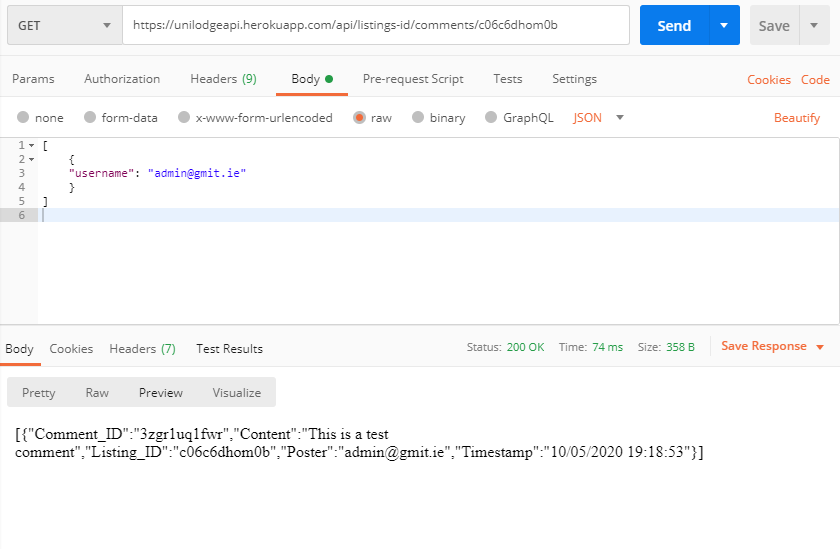
\includegraphics[width=0.70\textwidth]{images/postman_ex.png}
\end{figure}	

\subsection{System Testing}
Selenium was used to test the overall system functionality and to validate the overall application. Selenium tests were ran against both Firefox and Chrome to test the overall functionality.

\begin{figure}[H]
	\caption{Selenium Testing Functionality}
	\label{image:selenium}
	\centering
	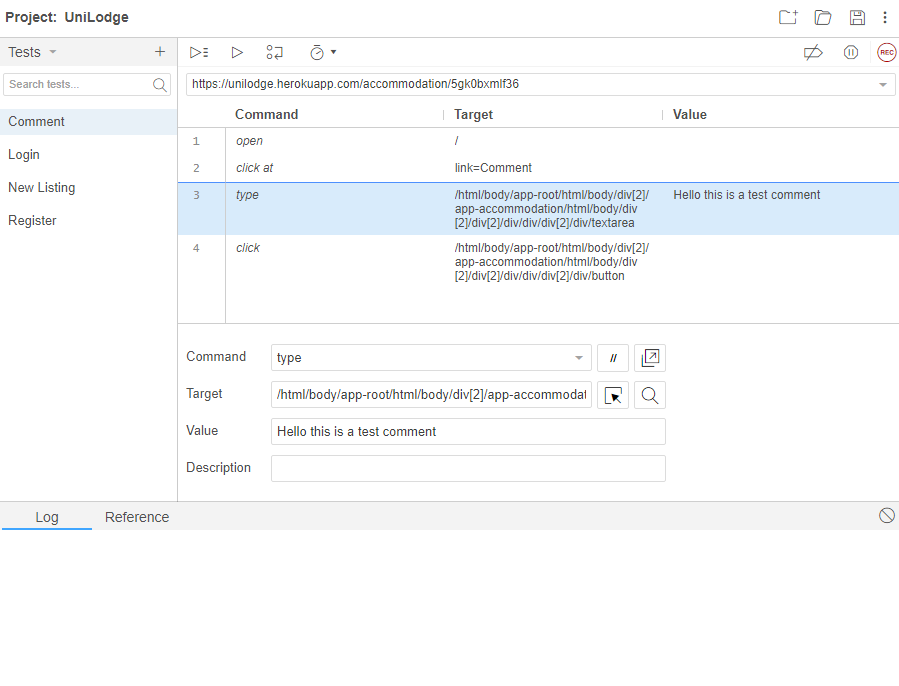
\includegraphics[width=0.70\textwidth]{images/selenium.png}
\end{figure}	

\paragraph{}
Selenium allowed the testing of vital functionality via automated clicks, input and submissions among other potential options. In \textbf{Figure 5.2}, a URL could be specified for Selenium to run the pre-written test against. By defining specific actions and elements to interact with by specifying their xpath, Selenium can automate an isolated test against the specified path to ensure it functions as expected.

\section{Limitations and Opportunities for Improvement}
While the proposed objectives for the project were achieved, there are still multiple areas within the developed system that can be vastly improved.

\subsection{Testing}
Although periodic unit testing with Karma, Jasmine and Selenium was conducted and usability tests were incorporated along with acceptance and verification testing to validate the project objectives, overall testing could have been a lot more prevalent throughout the system.

\paragraph{}
Unit Testing wasn't as abundant as it should have been, however during the early stages of development Karma and Jasmine were utilized at an acceptable level to ensure functionality like navigation and intractable components worked as intended. With that said, System Testing was an area of testing that really fell short during the project life-cycle.

\paragraph{}
System testing earlier in the development life cycle would have identified the issue of Flask not correctly serving Angular build files. Angular build files weren't generated until time came to deploy the application, so Flask only ever served development files. Build files were required for Heroku to be able to host the application, meaning the workaround was necessary, but could have been avoided if system tests were incorporated earlier and builds were generated periodically to test deployment. If this was carried out, the issue with Flask would have been able to be addressed much earlier in the development cycle.

\subsection{Lack of Additional Functionality}
The developed system, while adhering to the outlined goals, does lack in the area of additional user functionality that would see it be a serious alternative to applications of a similar nature.

\newpage

\paragraph{}
Features like profile enhancements, additional user functionality and the overall aesthetic of the application are on the list of future enhancements that will see implementation in future development cycles.

\subsection{Device Portability}
Following deployment, the application was tested on mobile, and while it works, the overall display of pages and components isn't ideal and can be improved upon. This can be solved in future by including some media and device responsive CSS on the most problematic pages.

\paragraph{}
This could have been addressed during development by consistently testing the application on alternative devices, however this was never a priority or an objective. In the future it would absolutely correct the cross-device aesthetic of the application.

\subsection{API Request Speed}
Something that the team had attempted to address at multiple points during the development cycle is the stuttering of some API interactions. This delay would result in components loading faster than the API data could be retrieved, an undesirable feature that isn't pleasant to see in an application. 

\paragraph{}
Different methods like lazy loading and progress / loading bars were trialed and implemented to attempt to address the inconvenience, however, while it was mostly corrected with the aforementioned methods, it does still remain a slight problem with the application with some components more than others.

\section{Overall Evaluation}
Overall the system functions as was intended, a platform for both students searching for and offering accommodate services. The requirements outlined in \textbf{Section 1.1}. Even though much was accomplished, the importance of testing in a system of this scale was learned, regardless if in terms of industry standard systems the developed application is minuscule in comparison, it only highlights the importance of maintainability during development.

\paragraph{}
With that being said, not extensively testing did yield a silver lining, the team did learn how to overcome unexpected issues that may arise and find unique solutions that wouldn't traditionally be sought out.

\paragraph{}
Finally, the overall development stack is considered by the team a worthy choice. The fact it was diverse stack not only enhanced knowledge of the individual components, but also first-hand experience on how to wire technologies together that wouldn't traditionally be coupled is a valuable learning outcome that can be applied to future projects. 

